\documentclass[10pt]{article}
\usepackage{tmlr}
% Camera-ready: \usepackage[accepted]{tmlr}   Preprint: \usepackage[preprint]{tmlr}

\usepackage{amsmath,amssymb,amsthm}
\usepackage{hyperref}
\usepackage{url}
\usepackage{booktabs}
\usepackage{graphicx}
\usepackage{xcolor}
\usepackage{enumitem}

% ---------------------------------------------------------------------------
% Pre-submission markers. Every \needed{} must be resolved (or the sentence
% removed) before submission; set \showneededfalse only after that.
\newif\ifshowneeded \showneededfalse
\newcommand{\needed}[1]{\ifshowneeded\textcolor{red}{\textbf{[#1]}}\fi}
% ---------------------------------------------------------------------------

\newtheorem{theorem}{Theorem}
\newtheorem{corollary}[theorem]{Corollary}
\newtheorem{proposition}[theorem]{Proposition}
\newtheorem{lemma}[theorem]{Lemma}
\theoremstyle{definition}
\newtheorem{definition}{Definition}
\newtheorem{example}{Example}
\theoremstyle{remark}
\newtheorem{remark}{Remark}

\newcommand{\X}{\mathcal{X}}
\newcommand{\A}{\mathcal{A}}
\newcommand{\R}{\mathbb{R}}
\newcommand{\conf}{c}
\newcommand{\dF}{\delta_{\!F}}
\newcommand{\leanid}[1]{{\def\_{\textunderscore\allowbreak}\texttt{#1}}}
\newcommand{\mech}{\textsc{m}}   % mechanized in Lean
\newcommand{\paper}{\textsc{p}}  % proved on paper only

\title{Truth Has a Boundary: A Machine-Checked Coupling Between\\
Truth and Confidence under Connectedness and Exact Separation}

\author{Anonymous authors\\Paper under double-blind review}

\def\month{MM}
\def\year{YYYY}
\def\openreview{\url{https://openreview.net/forum?id=XXXX}}

\begin{document}
\maketitle

\begin{abstract}
Probing studies read truth-related signals from language-model
activations with continuous readouts. We ask what follows when a truth
readout $\dF$ and a confidence signal $\conf$ are treated as continuous
fields on a connected representation space. The answer splits in two.
Exact pointwise separation (confidence above a threshold $\tau$ wherever
the answer is strictly true, and below $\tau$ wherever it is strictly
false) forces the confidence level set $\{\conf=\tau\}$ into the truth
boundary $\{\dF=0\}$, with no topology at all. Connectedness, continuity
and coverage make $\{\conf=\tau\}$ nonempty. Together they yield a query
with confidence exactly $\tau$ and truth-distance exactly zero, so a
threshold-inclusive truth guarantee is inconsistent with these premises,
while a threshold-exclusive one is consistent but silent at that query.
We derive quantitative, geometric, symmetry and discrete relaxations and
machine-check the core results in Lean~4 with Mathlib, marking the few
steps proved only on paper. Because the theorems need no empirical test,
our experiments measure their demanding premise instead. In five open
language models of up to 1.5B parameters, along interpolation paths from
true city statements to their negations, no path is exactly separated by
two independently trained linear readouts, and the smallest truth slack
that restores separation on a path has a median of 0.10 to 0.44 of the
truth field's scale. Across the five models, probe accuracy and median
slack have the same rank ordering, though nonlinear readouts and the
paths on which both readouts classify the endpoints correctly only partly
preserve it. The model's own confidence is at least as far from the
premise (median slack 0.12 to 0.91). The coupled query itself is not
observable with these paths, which confound truth with negation.
\end{abstract}

% ===========================================================================
\section{Introduction}
\label{sec:intro}

Linear probes recover truth-related directions from language-model
activations, and steering along such directions changes model behaviour
\citep{marks2024geometry,azaria2023internal,li2023inference,zou2023representation,burger2024truth}.
These pipelines apply a continuous readout at arbitrary points of an
activation space, including interpolated and edited activations that no
prompt produced. Whether such readouts track semantic truth is contested
\citep{farquhar2023challenges,levinstein2024still}; we do not settle that
question. We ask a narrower one: \emph{if} a truth readout and a
confidence signal are continuous fields on a connected space, what must
hold of them jointly?

The obstacle to a clean answer is that ``a model cannot be both
confident and right everywhere'' is either false or vacuous unless every
premise is stated. Existing inevitability results for hallucination are
statistical or computability-theoretic
\citep{kalai2024calibrated,xu2024hallucination,karbasi2025impossibility}
and say nothing about where in representation space the difficulty
sits.

Our observation is that the question decomposes. \emph{Alignment} of the
two fields' level sets is a pointwise consequence of separation: exact
separation alone forces $\{\conf=\tau\}\subseteq\{\dF=0\}$
(Proposition~\ref{prop:containment}). \emph{Existence} is where topology
enters: connectedness, continuity of $\conf$ and coverage make
$\{\conf=\tau\}$ nonempty. The mathematics is elementary, and we say so;
its value is that each premise does one identifiable job, and that the
conclusion mentions no safety guarantee and no threshold convention, so
the different guarantee conventions become corollaries of one statement.

Concretely, combining the two halves gives the \emph{boundary coupling
theorem} (Theorem~\ref{thm:coupling}): some query has confidence exactly
$\tau$ and lies exactly on the truth boundary. We then relax each premise
and price the relaxation, and we mechanize the results in Lean~4.

Empirically, the theorem needs no test, since it holds whenever its
premises hold. What can be measured is how far real readouts are from
its demanding premise, exact separation, using the truth slack of
Theorem~\ref{thm:approx} measured path by path. In five open models no
path is exactly separated, and the per-path slack has the same rank
ordering as probe accuracy across the five linear readouts
(Table~\ref{tab:main}); the model's own confidence is at least as far from
the premise (Table~\ref{tab:endo}). Whether the coupled query can be observed
directly is a separate question, and with the available paths the answer
is no (Section~\ref{sec:observe}).

\paragraph{Contributions.}
\begin{enumerate}[leftmargin=*,itemsep=1pt,topsep=2pt]
\item \textbf{Boundary containment and coupling, with a guarantee
taxonomy.} Exact separation forces $\{\conf=\tau\}\subseteq\{\dF=0\}$;
connectedness, continuous confidence and coverage make the left side
nonempty, so some query has $\conf=\tau$ and $\dF=0$. Hence a threshold-inclusive
truth guarantee is inconsistent with these premises, and a
threshold-exclusive guarantee is consistent but silent at that query
(Section~\ref{sec:coupling}).
\item \textbf{Priced relaxations, mechanized.} Positive truth slack is
forced under an inclusive guarantee, Lipschitz corridor and tube bounds
hold around the coupled query, probe boundaries are hyperplanes exactly
(linear) or to first order (differentiable), symmetry can replace
coverage, and a discrete analysis shows that connectedness is what
supplies the boundary query (Sections~\ref{sec:geometry}--\ref{sec:discrete}).
Several of these transfer variants of the continuity argument of
\citet{bhatt2026defense} to two fields. All main statements are checked in Lean~4 (Table~\ref{tab:lean}), and
the few paper-only steps are marked.
\item \textbf{A measurement of the separation premise.} In five open
models we estimate the empirical truth slack and the fraction of points
violating separation, for trained linear and MLP readouts and for the
model's own confidence, with bootstrap intervals over paths. The results
are descriptive (one data split, one fit per readout), and we show that
the coupled query is not observable with true-to-negation paths
(Section~\ref{sec:experiments}).
\end{enumerate}

\paragraph{What we do not claim.}
The theorems do not bound error rates, do not assert that deployed
models are continuous or that their reachable inputs form a connected
set, and do not show that any probe tracks semantic truth. The coupled
query may be an activation that no prompt produces
(Section~\ref{sec:limits}). The experiments do not test the theorems,
which are mathematical consequences of their premises, and they do not
show the coupled query in any model; they quantify how far five small
models are from the separation premise on one family of statements, from
a single data split and a single fit per readout. Only Theorem~\ref{thm:dichotomy} concludes that strictly
false answers occur, and it does so under its own probabilistic
hypotheses.

% ===========================================================================
\section{Related work}
\label{sec:related}

\paragraph{Inevitability of hallucination.}
\citet{kalai2024calibrated} prove that, for arbitrary facts not
determinable from training data, a generatively calibrated language
model's hallucination rate is lower-bounded, with high probability, by
roughly the fraction of facts seen exactly once in training (a
Good--Turing missing-mass estimate) minus its miscalibration.
\citet{kalai2025why} argue that hallucinations arise as classification
errors and persist because evaluations reward guessing.
\citet{xu2024hallucination} prove inevitability for computable models by
diagonalization, \citet{banerjee2024llms} argue for it from
undecidability, \citet{karpowicz2025fundamental} derive an impossibility
for hallucination control from mechanism design, and
\citet{karbasi2025impossibility} show, in an identification-in-the-limit
framework, that hallucination detection from positive examples alone is
impossible for most language collections and becomes possible with
labelled negative examples. These results are
rate-level, distributional or computational. Ours is topological,
conditions on a continuous confidence field over a representation space,
and exhibits at least one query at which the obstruction sits; for the deterministic
results it yields exact uncertainty rather than confident falsehood.

\paragraph{Truth in representations.}
Truth-related signals are linearly decodable from activations
\citep{marks2024geometry,azaria2023internal}. Unsupervised probes have
been proposed \citep{burns2023discovering}, but they can recover
prominent non-truth features \citep{farquhar2023challenges}, and
supervised probes can fail to generalize, including under negation
\citep{levinstein2024still}. \citet{burger2024truth} report a
two-dimensional truth subspace containing a polarity-sensitive direction
whose sign flips under negation, which is the empirical motivation for
our oddness premise (Section~\ref{sec:antipodal}). Steering along learned
directions changes truthfulness \citep{li2023inference,zou2023representation},
and concepts are often modelled as directions \citep{park2024linear},
though some features are irreducibly multi-dimensional
\citep{engels2025not}. We take one premise of this programme, that a
probe defines a continuous field whose zero set separates its classes,
and derive what it implies jointly with a confidence field. Confidence
signals themselves are produced in several ways, including trained heads
over activations \citep{kadavath2022language} and entropy over sampled
generations \citep{farquhar2024detecting}; our theorems apply only to
confidence that is a continuous function of the representation.

\paragraph{Abstention and the inevitability of errors.}
Selective classification studies classifiers that may abstain, trading
coverage against risk \citep{chow1970optimum,elyaniv2010foundations,geifman2017selective}.
The inclusive and exclusive guarantees of Definition~\ref{def:premises}
are pointwise analogues of its risk constraints, and abstaining on a
region is exactly the escape from Theorem~\ref{thm:coupling} that
Section~\ref{sec:limits} describes, since removing an open region can
disconnect the domain. \citet{shafahi2019adversarial} show that, for data
on certain manifolds, adversarial examples are unavoidable for any
classifier, by concentration of measure; their result bounds the measure
of points near a decision boundary, while ours exhibits a point on it
under a separation premise.

\paragraph{Topological arguments in learning.}
\citet{bhatt2026defense} use a related continuity argument on a
connected prompt space to show that continuous, utility-preserving
prompt-injection wrappers cannot be complete, and mechanize it in
Lean~4, together with discrete, $\varepsilon$-relaxed, Lipschitz,
boundary-dimension, multi-turn and stochastic variants. The present work
transfers that argument and its variants to a pair of fields, truth and
confidence; in particular Theorem~\ref{thm:boundary},
Theorem~\ref{thm:closed} and Proposition~\ref{prop:discrete-ivt} restate
lemmas of that development for the composite field $\dF$. The
mathematical object differs: that work constrains a single continuous
transformation $D:\X\to\X$ (a defense wrapper) through one score
function, whereas this paper studies the compatibility of two scalar
fields $(\dF,\conf):\X\to\R^2$ and the forced relationship between
their level sets. The new elements are the level-set containment and
two-field coupling, the threshold-convention taxonomy, the symmetry and
hyperplane results, and the premise measurements. The
strict-versus-weak threshold distinction also appears there, in the form
that a fixed boundary point is not strictly below the threshold. Borsuk--Ulam-type arguments give
impossibility results for replicable learning \citep{chase2024local}; our
symmetry results are scalar relatives that need only the intermediate
value theorem \citep{borsuk1933drei,matousek2003using}. Topological
analyses of trained networks \citep{naitzat2020topology,hensel2021survey}
and geometric deep learning \citep{bronstein2021geometric} study or
engineer such structure; we derive constraints from it.

% ===========================================================================
\section{Setting}
\label{sec:setting}

Let $\X$ be a topological space of queries as the model represents them
(for example residual-stream states) and $\A$ a topological space of
answers.

\begin{definition}[Model, truth field]
\label{def:model}
A \emph{model} is a map $F=(a,\conf):\X\to\A\times\R$ with answer $a(x)$
and scalar confidence $\conf(x)$. A \emph{truth field} is a map
$\delta:\X\times\A\to\R$, read as a signed truth-distance: negative on
strictly true answers, positive on strictly false ones. Its zero set is
the \emph{truth boundary}, and the \emph{realized truth field} is
$\dF(x)=\delta(x,a(x))$.
\end{definition}

\begin{definition}[Premises]
\label{def:premises}
Fix a threshold $\tau\in\R$, a truth slack $\varepsilon\ge 0$ and a
confidence margin $\gamma\ge 0$.
\begin{enumerate}[label=(\textbf{\Alph*}),leftmargin=*,itemsep=1pt,topsep=2pt]
\item[(T)] \emph{Connectedness:} $\X$ is connected and nonempty.
\item[(C)] \emph{Continuity:} $\conf$ is continuous (some results also
require $a$ and $\delta$ to be continuous; each statement says which).
\item[(Cov$_\varepsilon$)] \emph{Coverage:} some $x$ has
$\dF(x)<-\varepsilon$ and some has $\dF(x)>\varepsilon$.
\item[(Sep$_{\varepsilon,\gamma}$)] \emph{Separation at $\tau$:}
$\dF(x)<-\varepsilon\Rightarrow\conf(x)>\tau+\gamma$ and
$\dF(x)>\varepsilon\Rightarrow\conf(x)<\tau-\gamma$ for all $x$.
\emph{Exact} separation is $\varepsilon=\gamma=0$.
\end{enumerate}
A \emph{threshold-inclusive guarantee} is
$\conf(x)\ge\tau\Rightarrow\dF(x)<0$ for all $x$; a
\emph{threshold-exclusive guarantee} is $\conf(x)>\tau\Rightarrow\dF(x)<0$.
\end{definition}

\paragraph{Status of the premises.}
Each premise is an idealization, and we flag the evidence against each.
\emph{(T)} holds for ambient spaces such as $\R^d$, which is where probes
and steering vectors are applied. The set of activations reachable from
actual prompts is finite, and contextual embeddings show clustered
structure \citep{cai2021isotropy}; Section~\ref{sec:discrete} prices
dropping (T) and says where a language model does and does not meet it. \emph{(C)} holds for compositions of continuous layers but
fails at argmax decoding. \emph{Coverage} holds for any model that is
sometimes right and sometimes wrong. \emph{Exact separation} is
pointwise and much stronger than statistical calibration
\citep{guo2017calibration}; it idealizes a perfect truth probe used as
confidence, and Section~\ref{sec:experiments} measures how far trained
readouts are from it. A linear probe $w^\top x-b$ is a continuous
candidate for $\dF$; whether its zero set matches semantic truth away
from training samples is an empirical premise, not a theorem.

\begin{remark}[Biconditional separation]
\label{rem:biconditional}
Some results use \emph{biconditional} separation at $\tfrac12$:
$\conf(x)>\tfrac12\Leftrightarrow\dF(x)<0$ and
$\conf(x)<\tfrac12\Leftrightarrow\dF(x)>0$. It implies exact one-way
separation at $\tfrac12$
(\leanid{strictCalibrated\_to\_epsCalibrated\_zero\_half}).
\end{remark}

% ===========================================================================
\section{Boundary containment and coupling}
\label{sec:coupling}

The central result has two halves, one pointwise and one topological.

\begin{center}
\fbox{\begin{minipage}{0.93\linewidth}
\begin{proposition}[Boundary containment]
\label{prop:containment}
Let $\X$ and $\A$ be arbitrary sets, $F=(a,\conf)$ and $\delta$ arbitrary
maps, and suppose exact separation (Sep$_{0,0}$) holds at $\tau$. Then
\[
\{x\in\X:\conf(x)=\tau\}\;\subseteq\;\{x\in\X:\dF(x)=0\}.
\]
No topology, continuity or coverage is used. Connectedness, continuity
of $\conf$ and coverage are what make the left-hand set nonempty
(Theorem~\ref{thm:coupling}).
\end{proposition}
\end{minipage}}
\end{center}

\begin{proof}
If $\conf(x)=\tau$ and $\dF(x)<0$, separation gives $\conf(x)>\tau$; if
$\dF(x)>0$, it gives $\conf(x)<\tau$. Both contradict $\conf(x)=\tau$, so
$\dF(x)=0$. This is the second half of the Lean proof of
\leanid{boundary\_coupling} (Appendix~\ref{app:leanproof}); it is not
stated there as a separate lemma.
\end{proof}

\begin{theorem}[Boundary existence]
\label{thm:boundary}
Assume (T), that $a$ and $\delta$ are continuous, and (Cov$_0$). Then
some $x_0\in\X$ has $\dF(x_0)=0$.
\end{theorem}
\begin{proof}
$\dF$ is continuous and takes both signs on a connected space, so the
intermediate value theorem (Mathlib's
\texttt{IsPreconnected.intermediate\_value\textsubscript{2}}) gives a
zero. Lean: \leanid{model\_truth\_boundary\_nonempty}.
\end{proof}

\begin{theorem}[Boundary coupling]
\label{thm:coupling}
Assume (T), (C), (Cov$_0$) and exact separation (Sep$_{0,0}$) at
$\tau$. Then $\{\conf=\tau\}$ is nonempty, so some $x_0\in\X$ satisfies
\[
\conf(x_0)=\tau\qquad\text{and}\qquad\dF(x_0)=0 .
\]
Neither $a$ nor $\delta$ needs to be continuous.
\end{theorem}
\begin{proof}
Separation turns the two coverage witnesses into points with
$\conf>\tau$ and $\conf<\tau$; the intermediate value theorem on the
connected space gives $x_0$ with $\conf(x_0)=\tau$, and
Proposition~\ref{prop:containment} gives $\dF(x_0)=0$. Lean:
\leanid{boundary\_coupling}; the proof term is in
Appendix~\ref{app:leanproof}.
\end{proof}

We call such an $x_0$ a \emph{coupled query}
(Figure~\ref{fig:schematic}). The theorem mentions no guarantee, so the
choice between inclusive and exclusive guarantees only selects which
corollary applies.

\begin{figure}[t]
\centering
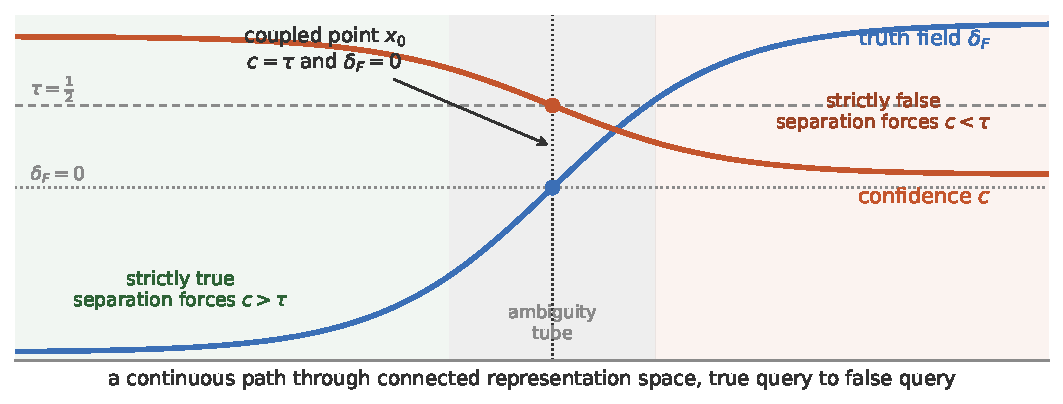
\includegraphics[width=0.6\linewidth]{schematic_coupling.pdf}
\caption{Schematic of Theorem~\ref{thm:coupling} (illustrative curves,
not data). Along a path from a strictly true to a strictly false query,
exact separation forces confidence above $\tau$ wherever $\dF<0$ and
below $\tau$ wherever $\dF>0$, so the two zero crossings coincide at the
coupled query $x_0$. The shaded band depicts the tube of
Theorem~\ref{thm:width}; its width here is drawn by hand, not computed.}
\label{fig:schematic}
\end{figure}

\begin{corollary}[Guarantee taxonomy]
\label{cor:policy}
Under the hypotheses of Theorem~\ref{thm:coupling}:
\begin{enumerate}[label=(\roman*),leftmargin=*,itemsep=1pt,topsep=2pt]
\item a threshold-inclusive guarantee at $\tau$ cannot also hold
(Lean: \leanid{closed\_guarantee\_impossible}; the $\tau=\tfrac12$,
biconditional special case, stated with additional unused continuity
hypotheses on $a$ and $\delta$, is \leanid{hallucination\_trilemma});
\item the coupled query $x_0$ has $\conf(x_0)=\tau$, so it does not
satisfy the antecedent $\conf(x_0)>\tau$ of a threshold-exclusive
guarantee (Lean: \leanid{open\_guarantee\_silent});
\item a threshold-exclusive guarantee is consistent with all hypotheses
(Example~\ref{ex:exclusive}; proved on paper, not mechanized).
\end{enumerate}
\end{corollary}

\begin{example}[An exclusive guarantee is satisfiable]
\label{ex:exclusive}
Let $\X=\A=\R$, $a(x)=x$, $\delta(x,y)=y$, $\tau=\tfrac12$ and
$\conf(x)=1/(1+e^{x})$, a probability. Then $\X$ is connected, $\conf$ is continuous,
$\dF(-1)<0<\dF(1)$; since $\conf(x)>\tfrac12$ exactly when $x<0$,
$\dF(x)<0\Leftrightarrow\conf(x)>\tfrac12$ and
$\dF(x)>0\Leftrightarrow\conf(x)<\tfrac12$, so exact (indeed
biconditional) separation holds. The exclusive guarantee holds because
$\conf(x)>\tfrac12$ implies $x<0$, that is, $\dF(x)<0$. The inclusive
guarantee fails at $x=0$, the coupled query. For a general threshold
$\tau$, the confidence $\conf(x)=\tau-\tfrac12+1/(1+e^{x})$ works the
same way, since $\conf(x)>\tau$ exactly when $x<0$.
\end{example}

The corollary is the paper's trilemma. Coverage, exact separation and an
inclusive guarantee cannot hold together on a connected space with
continuous confidence. Replacing $\ge$ by $>$ in the guarantee removes
the contradiction but not the coupled query.

% ===========================================================================
\section{Relaxations and the geometry of the boundary}
\label{sec:geometry}

\begin{theorem}[Approximate coupling; slack must be positive]
\label{thm:approx}
Assume (T), (C), (Cov$_\varepsilon$), (Sep$_{\varepsilon,\gamma}$) with
$\varepsilon,\gamma\ge0$, and a threshold-inclusive guarantee at $\tau$.
Then some $x_0$ has $\conf(x_0)=\tau$ and $-\varepsilon\le\dF(x_0)<0$.
Consequently $\varepsilon>0$: under these hypotheses exact truth slack
is infeasible for every confidence margin $\gamma\ge0$. Lean:
\leanid{two\_slack\_approx\_coupling},
\leanid{truth\_slack\_must\_be\_positive}; the $\varepsilon=0$ case is
\leanid{exact\_from\_approx}.
\end{theorem}

Theorem~\ref{thm:approx} says only that $\varepsilon=0$ is excluded. It
does not show that any particular $\varepsilon>0$ is achievable, and it
gives no positive lower bound on the infimum of feasible slack.

\begin{theorem}[Corridor and tube]
\label{thm:width}
Let $\X$ be a pseudometric space, $\conf$ $L_c$-Lipschitz and $\dF$
$L_\delta$-Lipschitz.
(i) If $L_c>0$, any $x,y$ with $\conf(x)\ge\tau+\gamma$ and
$\conf(y)\le\tau-\gamma$ satisfy $d(x,y)\ge 2\gamma/L_c$.
(ii) If $\conf(x_0)=\tau$, $\dF(x_0)=0$ and $L_c,L_\delta\ge0$, then every
$x$ with $d(x,x_0)\le r$ has $|\dF(x)|\le L_\delta r$ and
$|\conf(x)-\tau|\le L_c r$. Lean: \leanid{confidence\_gap\_width},
\leanid{truth\_margin\_tube}, \leanid{ambiguity\_tube}.
\end{theorem}

\begin{theorem}[Boundary sets]
\label{thm:closed}
For topological $\X,\A$ and continuous $a,\delta$, the set
$\{x:\dF(x)=0\}$ is closed, and for every continuous
$\gamma:\R\to\X$ and $s\le t$ with $\dF(\gamma(s))<0<\dF(\gamma(t))$ there
is $u\in[s,t]$ with $\dF(\gamma(u))=0$. No connectedness of $\X$ is
needed. Lean: \leanid{model\_truth\_boundary\_isClosed},
\leanid{path\_crosses\_truth\_boundary}.
\end{theorem}

\begin{theorem}[Probe boundaries are hyperplanes, exactly or to first order]
\label{thm:hyperplane}
Let $E$ be a real vector space of finite dimension $d$.
(i) Let $f:E\to\R$ be a nonzero linear map and $b\in\R$. Then
$\{f=b\}$ is nonempty and equals $x_0+\ker f$ for any $x_0$ with
$f(x_0)=b$, and $\dim\ker f=d-1$.
(ii) Let $E$ be normed, $f:E\to\R$ differentiable at $x_0$ with
$f(x_0)=0$ and derivative $L\ne0$. Then every ball around $x_0$ contains
points with $f>0$ and points with $f<0$; for every $\eta>0$ there is
$\rho>0$ such that every $x$ with $\|x-x_0\|<\rho$ and $f(x)=0$
satisfies $|L(x-x_0)|\le\eta\|x-x_0\|$; and $\dim\ker L=d-1$.
\end{theorem}
\begin{proof}
(i) Lean: \leanid{linear\_probe\_boundary\_coset} (coset form, given a
base point) and \leanid{linear\_probe\_boundary\_dim} (rank--nullity).
Nonemptiness is proved on paper: $f\ne0$ gives some $v$ with $f(v)\ne0$,
and $x_0=(b/f(v))\,v$ satisfies $f(x_0)=b$. (ii) Lean:
\leanid{regular\_point\_is\_crossing},
\leanid{nonlinear\_boundary\_tangent} (which needs neither $L\ne0$ nor
finite dimension), \leanid{tangent\_hyperplane\_dim}.
\end{proof}

For the probes used in practice, therefore, the zero set of $\dF$ that
Theorem~\ref{thm:coupling} places a coupled query on is an affine
hyperplane, or near a regular point a set that deviates sublinearly from
its tangent hyperplane.

% ===========================================================================
\section{Symmetry can replace coverage}
\label{sec:antipodal}

Suppose negation acts on $\X$ as a continuous involution $\sigma$ without
fixed points and the realized truth field is odd,
$\dF(\sigma x)=-\dF(x)$. This idealizes the polarity-sensitive truth
direction reported by \citet{burger2024truth}; probes trained on
affirmative statements need not generalize to negations
\citep{levinstein2024still}, and Section~\ref{sec:experiments} measures
the deviation from oddness.

\begin{theorem}[Odd fields vanish]
\label{thm:odd-zero}
If $\X$ satisfies (T) and carries such an involution $\sigma$, every
continuous $g:\X\to\R$ with $g\circ\sigma=-g$ has a zero. The proof uses
only oddness and the intermediate value theorem between $x$ and
$\sigma x$. Lean: \leanid{antipodal\_odd\_has\_zero}.
\end{theorem}

\begin{theorem}[Approximate and spherical oddness]
\label{thm:approx-odd}
(i) If $\X$ satisfies (T), $\sigma:\X\to\X$ is any map, and $g$ is
continuous with $|g(\sigma x)+g(x)|\le\varepsilon$ for \emph{all} $x$,
then some $x$ has $|g(x)|\le\varepsilon/2$.
(ii) For $d\ge2$, every function on $\R^d$ that is continuous on the unit
sphere and odd there under $x\mapsto-x$ vanishes somewhere on the
sphere. Lean: \leanid{approx\_odd\_near\_zero},
\leanid{sphere\_odd\_has\_zero}.
\end{theorem}

\begin{theorem}[Antipodal coupling]
\label{thm:antipodal}
Assume (T), a continuous fixed-point-free involution $\sigma$, continuous
$a$, $\delta$ and $\conf$ (the last is assumed in the Lean statement but
unused), $\dF$ odd under $\sigma$, and biconditional separation
at $\tfrac12$. Then some $x$ has $\conf(x)=\tfrac12$ and $\dF(x)=0$. No
coverage hypothesis appears. Lean:
\leanid{antipodal\_hallucination\_trilemma}.
\end{theorem}

These are scalar relatives of Borsuk--Ulam; no Borsuk--Ulam theorem is
used in the proofs. Theorem~\ref{thm:approx-odd}(ii) is stated for the
Euclidean unit sphere only. Normalization layers map hidden states close
to a sphere up to a learned affine map, but this connection is
interpretation and is not formalized.

% ===========================================================================
\section{Without the continuum; turns and randomness}
\label{sec:discrete}

Token sequences are discrete. The following results show what remains
when topology is removed: the boundary query must be assumed rather than
derived.

\begin{theorem}[Discrete impossibility]
\label{thm:discrete}
For arbitrary sets $\X,\A$ and arbitrary $F,\delta$ with biconditional
separation at $\tfrac12$: if some query has $\dF=0$, the inclusive
guarantee at $\tfrac12$ fails; and the inclusive guarantee holds if and
only if no query has $\dF=0$. Lean:
\leanid{boundary\_question\_impossible},
\leanid{faithful\_iff\_boundary\_free}.
\end{theorem}

\begin{proposition}[Discrete sign change]
\label{prop:discrete-ivt}
If $g:\{0,\dots,n\}\to\R$ has $g(0)<0<g(n)$, some $i<n$ has
$g(i)<0\le g(i+1)$. Lean: \leanid{discrete\_sign\_change}.
\end{proposition}

Along a sequence of token-level edits from a true to a false statement,
$\dF$ therefore changes sign between adjacent steps, but no step need sit
exactly on the boundary. Connectedness is what turns this straddling pair
into a boundary query (Theorem~\ref{thm:boundary}).

\paragraph{Where a language model meets the premises.}
For a dense transformer (without mixture-of-experts routing or activation
quantization, both of which are discontinuous), the map from a
fixed-length sequence of input embeddings, or from a hidden state at a
fixed position, to the next-token distribution is a composition of
continuous maps, so it is continuous on a connected space. Probes,
steering vectors, soft prompts and embedding-space attacks act at this
level, so there (T) and continuity of $\conf$ hold. Continuity of the
decoded answer $a$ does not, since decoding is an argmax or a sample, so
of the results above only those that need continuity of $\conf$ alone
(Theorem~\ref{thm:coupling}, Corollary~\ref{cor:policy}) apply without
further idealization. The realizable inputs are always finite: a text
prompt of bounded length has finitely many token sequences, and image or
audio inputs are quantized (for example 8-bit pixels), so the continuous
input space $[0,1]^n$ of such models is an idealization of the same kind,
on a finer grid. A coupled query therefore need not be the representation
of any realizable input, and a guarantee stated only over realizable
inputs is not contradicted by Theorem~\ref{thm:coupling}.
Theorem~\ref{thm:width} does not restore the contradiction. It says only
that if the realizable representations and a coupled query lie in a
bounded convex set on which $\conf$ and $\dF$ are $L_c$- and
$L_\delta$-Lipschitz (dot-product attention need not be globally
Lipschitz, so a bounded set is required), then a realizable input within
distance $r$ of the coupled query has $|\conf-\tau|\le L_c r$ and
$|\dF|\le L_\delta r$; under the slack of Theorem~\ref{thm:approx}, where
the coupled query only has $|\dF|\le\varepsilon$, the second bound becomes
$\varepsilon+L_\delta r$. How close realizable inputs come to coupled
queries is an empirical question we do not measure. In every case
coverage and exact separation remain premises.

\paragraph{Multiple turns.}
If a model maps a length-$T$ history in $\X^T$ to one answer and
confidence, $\X^T$ with the product topology is connected whenever $\X$
is. The $\tfrac12$-threshold biconditional form of
Corollary~\ref{cor:policy}(i) then applies, with the additional
continuity of $a$ and $\delta$ assumed in
\leanid{multi\_turn\_history\_dependent}. We have mechanized only this
statement for histories; per-turn answer sequences are not modelled.

\paragraph{Randomness.}
If the \emph{expected} confidence $\bar\conf$ and \emph{expected} truth
distance $\bar\delta$, viewed as functions of the query, satisfy (C),
coverage and exact separation at $\tfrac12$, Theorem~\ref{thm:coupling}
gives a query with $\bar\conf=\tfrac12$ and $\bar\delta=0$
(\leanid{stochastic\_coupling\_expected}). The Lean statement takes
$\bar\conf,\bar\delta$ as arbitrary functions; deriving their continuity
and separation from sample-level properties is not formalized. At such a
query the following holds.

\begin{theorem}[Stochastic dichotomy]
\label{thm:dichotomy}
Let $(\Omega,\mu)$ be a probability space and $c,d:\Omega\to\R$ with $d$
integrable and $\int d\,d\mu=0$. If $c\ge\tfrac12\Rightarrow d<0$ holds
$\mu$-almost everywhere and $\mu\{c\ge\tfrac12\}>0$, then
$\mu\{d>0\}>0$. Lean: \leanid{stochastic\_dichotomy}.
\end{theorem}

Read with $\Omega$ the sampling randomness at a fixed query whose
expected truth distance is zero, a sampler that is faithful on almost
every sample and confident with positive probability must emit strictly
false answers with positive probability. Instantiating $\Omega$ this way
is a modelling step that we have not formalized. At such a query the
hypothesis $\mu\{c\ge\tfrac12\}>0$ is automatic when $c$ is integrable
with mean $\tfrac12$: otherwise $c<\tfrac12$ almost surely, and its mean
would be strictly below $\tfrac12$ (paper proof, not mechanized).

% ===========================================================================
\section{Mechanization}
\label{sec:lean}

The Lean~4 \citep{moura2021lean} development, built on Mathlib
\citep{mathlib2020} (toolchain \texttt{v4.28.0}, Mathlib
\texttt{v4.28.0}, 18 source files plus a root module) states results over arbitrary
topological, pseudometric or normed spaces as each theorem requires.
Table~\ref{tab:lean} maps every statement in this paper to its Lean
identifier and marks whether it is mechanized (\mech) or proved on paper
only (\paper).

A search of the source finds no \texttt{sorry}, \texttt{admit},
\texttt{native\_decide} or \texttt{axiom} declarations. Several files
contain \texttt{\#print axioms} commands for main theorems, but we have
not recorded their output for every identifier in Table~\ref{tab:lean},
so we make no claim here about which axioms each theorem uses. The mechanized statements concern abstract spaces:
the identification of $\X$ with a model's representation space, of $\dF$
with a probe, and of $\sigma$ with negation is modelling, not
mechanized content.

\begin{table}[t]
\centering
\caption{Statements and their machine-checked counterparts. \mech:
mechanized in Lean; \paper: proved on paper only.}
\label{tab:lean}
\footnotesize
\begin{tabular}{@{}lcp{9.3cm}@{}}
\toprule
Result & Status & Lean identifier(s) \\
\midrule
Thm.~\ref{thm:boundary} & \mech & \leanid{model\_truth\_boundary\_nonempty} \\
Thm.~\ref{thm:coupling} & \mech & \leanid{boundary\_coupling} \\
Cor.~\ref{cor:policy}(i) & \mech & \leanid{closed\_guarantee\_impossible}; \leanid{hallucination\_trilemma} ($\tau=\tfrac12$, biconditional, continuous $a,\delta$) \\
Cor.~\ref{cor:policy}(ii) & \mech & \leanid{open\_guarantee\_silent} \\
Cor.~\ref{cor:policy}(iii) & \paper & Example~\ref{ex:exclusive} \\
Thm.~\ref{thm:approx} & \mech & \leanid{two\_slack\_approx\_coupling}, \leanid{truth\_slack\_must\_be\_positive}, \leanid{exact\_from\_approx} \\
Thm.~\ref{thm:width} & \mech & \leanid{confidence\_gap\_width}, \leanid{truth\_margin\_tube}, \leanid{ambiguity\_tube} \\
Thm.~\ref{thm:closed} & \mech & \leanid{model\_truth\_boundary\_isClosed}, \leanid{path\_crosses\_truth\_boundary} \\
Thm.~\ref{thm:hyperplane}(i) & \mech\,/\,\paper & \leanid{linear\_probe\_boundary\_coset}, \leanid{linear\_probe\_boundary\_dim}; nonemptiness on paper \\
Thm.~\ref{thm:hyperplane}(ii) & \mech & \leanid{regular\_point\_is\_crossing}, \leanid{nonlinear\_boundary\_tangent}, \leanid{tangent\_hyperplane\_dim} \\
Thm.~\ref{thm:odd-zero} & \mech & \leanid{antipodal\_odd\_has\_zero} \\
Thm.~\ref{thm:approx-odd} & \mech & \leanid{approx\_odd\_near\_zero}, \leanid{sphere\_odd\_has\_zero} \\
Thm.~\ref{thm:antipodal} & \mech & \leanid{antipodal\_hallucination\_trilemma} \\
Thm.~\ref{thm:discrete} & \mech & \leanid{boundary\_question\_impossible}, \leanid{faithful\_iff\_boundary\_free} \\
Prop.~\ref{prop:discrete-ivt} & \mech & \leanid{discrete\_sign\_change} \\
Multi-turn (Sec.~\ref{sec:discrete}) & \mech & \leanid{multi\_turn\_history\_dependent} ($\tfrac12$, biconditional, continuous $a,\delta$) \\
Expected fields (Sec.~\ref{sec:discrete}) & \mech & \leanid{stochastic\_coupling\_expected} (fields assumed, not derived) \\
Thm.~\ref{thm:dichotomy} & \mech & \leanid{stochastic\_dichotomy} \\
Prop.~\ref{prop:containment} & \mech\,/\,\paper & inside the proof of \leanid{boundary\_coupling}; not a standalone lemma \\
Dichotomy hypothesis automatic (Sec.~\ref{sec:discrete}) & \paper & -- \\
Rem.~\ref{rem:biconditional} & \mech & \leanid{strictCalibrated\_to\_epsCalibrated\_zero\_half} \\
\bottomrule
\end{tabular}
\end{table}

% ===========================================================================
\section{Measuring the separation premise in language models}
\label{sec:experiments}

\paragraph{What is measured, and why.}
Theorem~\ref{thm:coupling} holds whenever its premises hold, so it needs no
empirical test. What can be measured is how far real readouts are from its
one demanding premise, exact pointwise separation. The theory supplies the
unit: Theorem~\ref{thm:approx} relaxes separation by a truth slack
$\varepsilon$, and a readout pair is $(\varepsilon,0)$-separating exactly
when every point with $|\dF|>\varepsilon$ has its confidence on the
correct side of $\tfrac12$. Over the whole representation space this $\varepsilon$ is uninformative
for linear readouts: unless the two readouts' decision hyperplanes
coincide, the head's hyperplane $\{\conf=\tfrac12\}$ contains points with
arbitrarily large $|\dF|$, so no finite $\varepsilon$ works on $\R^d$. We
therefore measure it on a specified domain, the interpolation segments
between test statements: for each path we compute the smallest
$\varepsilon$ for which separation holds on that path, and we report its
median and its maximum over paths, together with the fraction of points
at which separation fails. The maximum over paths is the theory's
$\varepsilon$ restricted to the union of the measured segments. These are
measurements of a hypothesis, not tests of a prediction, so they need no
null model. Section~\ref{sec:observe} asks the separate question of
whether the coupled query itself is observable with this design; the
answer is no.

\subsection{Setup}
\label{sec:setup}

\textbf{Models:} GPT-2 (124M), Pythia-410M, Qwen2.5-0.5B, Phi-1.5 (1.3B)
and Qwen2.5-1.5B (Hugging Face ids in Appendix~\ref{app:exp}).
\textbf{Data:} the \texttt{cities} and \texttt{neg\_cities} statements of
\citet{marks2024geometry}, 1{,}496 statements each over 748 cities, each
statement paired with its negation of opposite label, split by city into
training split A (50\%), split B (20\%), validation (10\%) and test (20\%).
\textbf{Representation:} the final-token hidden state at one layer, chosen
by validation accuracy among $\{\lfloor n/4\rfloor,\lfloor n/2\rfloor,
\lfloor 3n/4\rfloor\}$ for an $n$-layer model.
\textbf{Fields:} $\dF$ is the negated logit of a standardized logistic
probe trained on split A. Confidence $\conf$ is either a second logistic
head trained on split B (\emph{trained confidence}; the two readouts share
no training statements but read the same representation), or the model's
own probability of the token ``true'' (\emph{endogenous confidence},
Section~\ref{sec:endo}). One training run of each readout was made.
In the notation of Section~\ref{sec:setting}, a query $x$ is the hidden
state of a statement, the ``answer'' $a(x)$ is the statement itself, and
$\dF(x)$ is the probe's signed estimate of that statement's truth; the
experiments therefore concern a readout of the input's truth, not the
truth of a generated answer.
\textbf{Paths:} for each of the 149 test cities whose affirmative
statement is true, the hidden state is interpolated linearly from that
statement to its negation at 41 points. Paths whose endpoints the probe
misclassifies are dropped, since the premise is only defined relative to
a probe that gets the endpoints right.
\textbf{Statistics, per path:} the \emph{violation fraction}, the share of
points where $\dF<0$ but $\conf\le\tfrac12$, or $\dF>0$ but
$\conf\ge\tfrac12$; whether the path is \emph{exactly separated} (no
violating point); and the \emph{empirical truth slack} $\hat\varepsilon$,
the largest $|\dF|$ among violating points divided by the endpoint scale
$\max(|\dF(\text{start})|,|\dF(\text{end})|)$, which is the smallest
$\varepsilon$ for which $(\varepsilon,0)$-separation holds on the path
($\hat\varepsilon=0$ if none). For linear readouts $\dF$ and the logit of
$\conf$ are affine along a straight path, so each path is determined
exactly by its endpoint values (reconstruction reproduces the saved
curves to within $4\times10^{-5}$ in the logit), and we evaluate it on
4{,}001 points; a coarse grid understates violations near the crossings.
MLP and endogenous readouts are not affine, and only their 41-point
curves were saved, so their statistics use 41 points. We report means
and medians over paths with percentile bootstrap 95\% intervals (10{,}000
path resamples), conditional on the trained readouts.

\subsection{Trained confidence}
\label{sec:main}

\begin{table}[t]
\centering
\caption{Separation premise between two independently trained linear
readouts, evaluated exactly at 4{,}001 points per path. \emph{Probe},
\emph{Head}: test accuracy of $\dF$ and $\conf$. \emph{Paths}: paths
whose endpoints the probe classifies correctly, of 149; none is exactly
separated. \emph{Head err.}: fraction of paths on which the head is on
the wrong side of $\tfrac12$ at an endpoint. \emph{Violation}: mean
fraction of violating points per path. $\hat\varepsilon$: median and
maximum empirical truth slack, in units of the endpoint scale.
$\hat\varepsilon\mid$ends: median slack on paths without a head endpoint
error. 95\% bootstrap intervals in brackets. Sources:
\texttt{results.json}, \texttt{results\_separation\_fine.json}.}
\label{tab:main}
\footnotesize
\setlength{\tabcolsep}{3.5pt}
\begin{tabular}{@{}lcccccccc@{}}
\toprule
Model & Layer & Probe & Head & Paths & Head err. & Violation & $\hat\varepsilon$ median / max & $\hat\varepsilon\mid$ends \\
\midrule
Phi-1.5 (1.3B) & 18/24 & 0.72 & 0.72 & 66/149  & 0.35 & 0.35 [0.29, 0.40] & 0.44 [0.33, 0.59] / 1.00 & 0.32 [0.21, 0.42] \\
GPT-2 (124M)   & 9/12  & 0.77 & 0.72 & 83/149  & 0.27 & 0.29 [0.24, 0.34] & 0.38 [0.23, 0.47] / 1.00 & 0.24 [0.17, 0.38] \\
Pythia-410M    & 18/24 & 0.82 & 0.77 & 104/149 & 0.26 & 0.28 [0.23, 0.32] & 0.30 [0.23, 0.43] / 1.00 & 0.25 [0.20, 0.37] \\
Qwen2.5-0.5B   & 12/24 & 0.96 & 0.96 & 137/149 & 0.04 & 0.15 [0.12, 0.17] & 0.18 [0.14, 0.20] / 1.00 & 0.18 [0.13, 0.19] \\
Qwen2.5-1.5B   & 14/28 & 1.00 & 1.00 & 148/149 & 0.00 & 0.07 [0.06, 0.08] & 0.10 [0.08, 0.12] / 0.78 & 0.10 [0.08, 0.12] \\
\bottomrule
\end{tabular}
\end{table}

\begin{figure}[t]
\centering
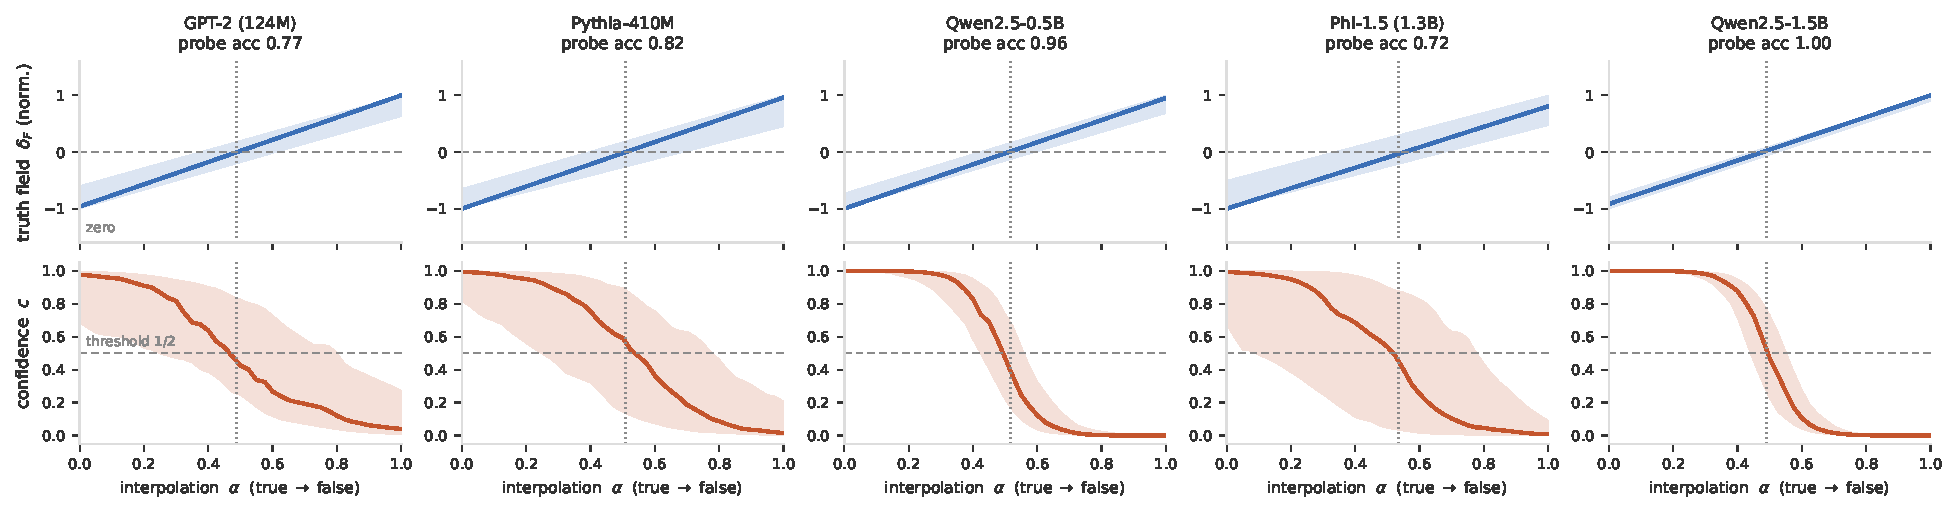
\includegraphics[width=\linewidth]{boundary_coupling.pdf}
\caption{Trained linear readouts along true-to-negation paths (median and
interquartile band over kept paths). Top: probe $\dF$ divided by the
endpoint scale. Bottom: trained head $\conf$. Dotted line: mean position
of the probe's zero crossing. Under exact separation the bottom curve
would cross $\tfrac12$ exactly at the dotted line on every path; the
spread around it is the separation violation measured in
Table~\ref{tab:main}.}
\label{fig:coupling}
\end{figure}

\textbf{RQ.} How far from exact separation are two independently trained
truth readouts of the same representation?
\textbf{Result} (Table~\ref{tab:main}). No path is exactly separated in
any model. The premise fails at 7\% to 35\% of path points on average,
and the median empirical truth slack is 0.10 to 0.44 of the endpoint
scale; the maximum over paths, which is the theory's $\varepsilon$ on the
measured segments, is the full endpoint scale in four models and 0.78 in
Qwen2.5-1.5B. Across the five models, probe accuracy, violation fraction
and median slack have the same rank ordering, though the bootstrap
intervals of the three weaker models overlap. Part of this ordering is
mechanical: where the head is on the wrong side of $\tfrac12$ at an
endpoint, the slack is large by construction (median 0.66 to 1.00), and
such paths are more common for less accurate heads (35\% for Phi-1.5,
none for Qwen2.5-1.5B). On the remaining paths the median slack is 0.10
to 0.32 and GPT-2 and Pythia-410M tie, so the ordering there separates the
two Qwen models from the other three rather than ranking all five. Since
the confidence head is itself a second truth probe on the same features,
this residual slack measures how far two logistic fits of the same target
disagree near their boundaries. These are descriptive observations about
five fits, not an estimated relationship, and the MLP readouts of
Section~\ref{sec:robust} only partly preserve them
(\texttt{results\_separation\_fine.json}).
\textbf{Relation to the theory.} The measured slack is strictly positive
in every model, which is what Theorem~\ref{thm:approx} requires of any
system that also carries an inclusive guarantee. That is consistency, not
confirmation: these readouts carry no such guarantee, and positive slack
would be expected of imperfect readouts in any case.
\textbf{Does not establish.} Five models give a rank ordering, not a
statistical trend, from a single data split and a single fit per readout.
Parameter count is not the ordering variable: Phi-1.5 is the
second-largest model but has the weakest probe, and a sweep over all its
layers on raw statements reaches at most 0.73 test accuracy (a probe on
its final-block states under the question template of
Section~\ref{sec:endo} reaches 0.78, so this is a property of the raw
representation, not a ceiling for the model).

\paragraph{Where separation fails.}
At the probe's zero crossing, the trained confidence is usually far from
$\tfrac12$: only 17\%, 10\%, 11\%, 5\% and 21\% of crossings (GPT-2,
Pythia-410M, Qwen2.5-0.5B, Phi-1.5, Qwen2.5-1.5B) have
$\conf\in[0.4,0.6]$, and 31\%, 43\%, 40\%, 67\% and 17\% have $\conf<0.1$
or $\conf>0.9$ (\texttt{results\_crossing\_conf.json}). The distribution
is widely dispersed, and U-shaped for Pythia-410M, Qwen2.5-0.5B and
Phi-1.5. The mean confidence at the crossing (0.52, 0.51, 0.49, 0.43,
0.54) is therefore not informative on its own.

\subsection{The model's own confidence}
\label{sec:endo}

\begin{table}[t]
\centering
\caption{Separation premise with endogenous confidence: the model's own
probability of the token ``true'' under a question template, read after
patching interpolated final-block states. \emph{Probe}: test accuracy of a
probe trained on the same final-block states. \emph{Paths}: paths whose
endpoints that probe classifies correctly, of 149. \emph{End.\ sep.}:
paths whose confidence is on the correct side of $\tfrac12$ at both
endpoints. Other columns as in Table~\ref{tab:main}. Sources:
\texttt{results\_endogenous.json}, \texttt{results\_separation.json}.}
\label{tab:endo}
\footnotesize
\begin{tabular}{@{}lcccccc@{}}
\toprule
Model & Probe & Paths & End.\ sep. & Exact & Violation & $\hat\varepsilon$ \\
\midrule
GPT-2 (124M)   & 0.66 & 53/149  & 23 (0.43)  & 0.00 & 0.41 [0.33, 0.49] & 0.60 [0.28, 0.85] \\
Pythia-410M    & 0.76 & 84/149  & 0 (0.00)   & 0.00 & 0.49 [0.44, 0.54] & 0.91 [0.79, 1.00] \\
Qwen2.5-0.5B   & 0.94 & 137/149 & 128 (0.93) & 0.08 & 0.18 [0.15, 0.21] & 0.18 [0.14, 0.25] \\
Phi-1.5 (1.3B) & 0.78 & 80/149  & 53 (0.66)  & 0.00 & 0.41 [0.36, 0.46] & 0.66 [0.53, 0.77] \\
Qwen2.5-1.5B   & 1.00 & 147/149 & 146 (0.99) & 0.08 & 0.10 [0.09, 0.11] & 0.12 [0.08, 0.16] \\
\bottomrule
\end{tabular}
\end{table}

\begin{figure}[t]
\centering
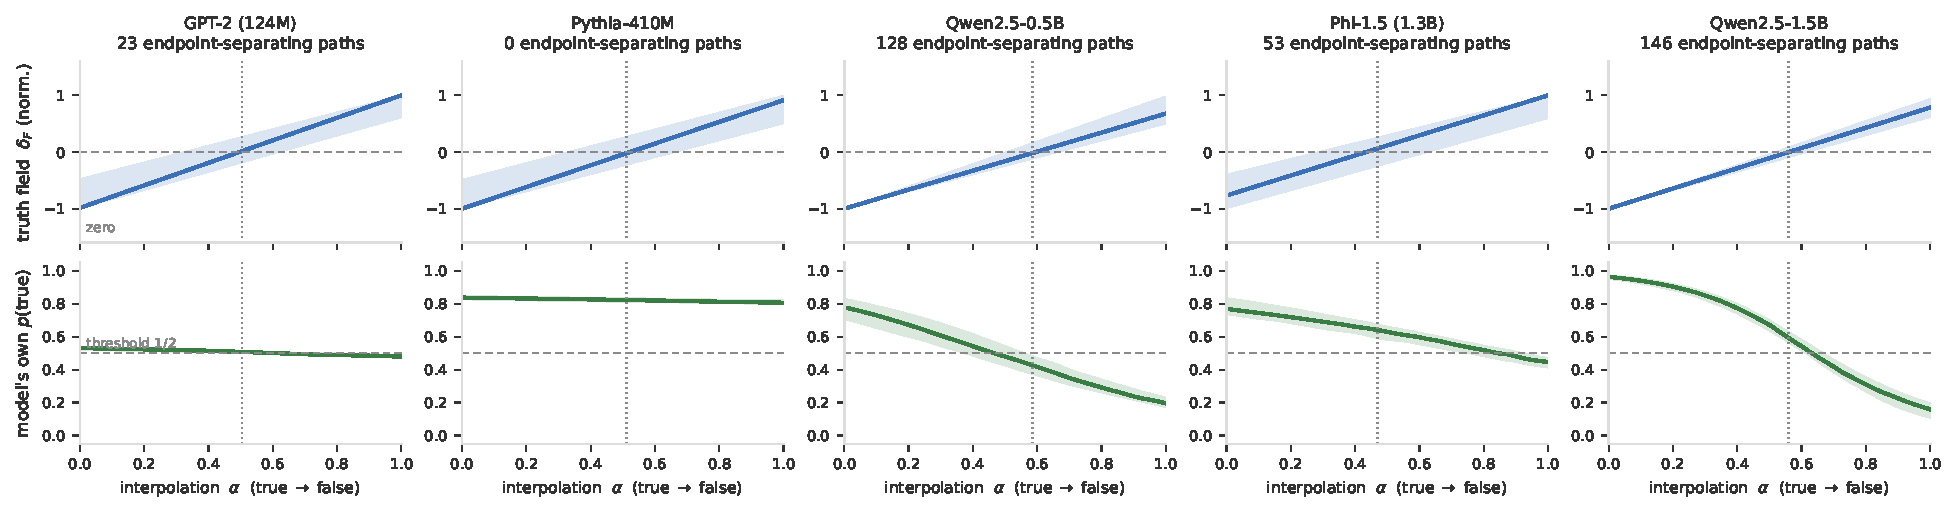
\includegraphics[width=\linewidth]{endogenous_coupling.pdf}
\caption{Endogenous confidence on endpoint-separating paths (all kept
paths for Pythia-410M, which has none). Top: probe $\dF$ on final-block
states, normalized by endpoint scale. Bottom: the model's own
$p(\text{true})$ on a common $[0,1]$ axis. Dotted line: mean probe zero
crossing. Only the two Qwen models sweep through $\tfrac12$ near the
probe's crossing; Phi-1.5 crosses late, GPT-2 stays near $\tfrac12$
throughout, and Pythia-410M stays above it.}
\label{fig:endo}
\end{figure}

\textbf{RQ.} Both readouts in Section~\ref{sec:main} are trained to
predict truth. How far is the model's own next-token confidence from the
premise?
\textbf{Setup.} Statements are wrapped in the template ``Q: Is this
statement true or false? \ldots{} A: The statement is''. We interpolate
the last-token output of the final transformer block, patch it in, and
read $p(\text{``true''})$ against $p(\text{``false''})$ through the final
normalization and unembedding; the probe is trained on split A of the same
final-block states.
\textbf{Result} (Table~\ref{tab:endo}, Figure~\ref{fig:endo}). Endogenous
confidence (statistics on the saved 41-point curves) is at least as far
from the premise as trained confidence in every model, and clearly
further in GPT-2, Pythia-410M and Phi-1.5; for Qwen2.5-0.5B the two
overlap (median slack 0.18 [0.14, 0.25] against 0.16 [0.11, 0.18] on the
same grid). The comparison is indirect, since the endogenous experiment
uses a different representation, probe and set of kept paths. Endogenous
confidence comes closest in the two Qwen models (median slack 0.12 and
0.18, violation at 10\% and 18\% of points), which are also the only
models whose confidence is on the correct side at both endpoints on more
than 90\% of paths. For Pythia-410M, whose confidence exceeds $\tfrac12$
everywhere, the premise fails at about half of all points and the slack is
close to the full endpoint scale. Phi-1.5 shows that endpoint agreement
is a weak proxy for the premise: its confidence is on the correct side at
both ends of 66\% of paths, yet it crosses $\tfrac12$ late on the path,
and its slack (0.66) is the second largest.
\textbf{Does not establish.} The endogenous confidence is a near-linear
readout (normalization, then a two-token unembedding difference) of the
same state the probe reads, so it is not independent of the
representation.

\subsection{Robustness}
\label{sec:robust}

\paragraph{Nonlinear readouts.}
With one-hidden-layer MLP readouts (64 units, early stopping) on the same
splits, probe accuracies are 0.79, 0.87, 0.97, 0.80 and 0.995 (GPT-2,
Pythia-410M, Qwen2.5-0.5B, Phi-1.5, Qwen2.5-1.5B), and 98\% or more of
kept paths cross zero exactly once. The median slack is 0.35, 0.41, 0.21,
0.34 and 0.09, and the violation fraction 0.22, 0.29, 0.13, 0.26 and 0.06
(41-point curves; \texttt{results\_separation.json}). The two Qwen models
are again closest to the premise. Among the other three the order differs from the
linear case: Pythia-410M has the most accurate MLP probe of the three but
the largest slack.

\paragraph{Unmatched paths.}
The affine reconstruction also gives paths from the true affirmative of
one test city to the negation of a different city, removing the matched
pairing (4{,}290 to 21{,}756 paths per model;
\texttt{compute\_separation\_fine.py}). These paths recombine the same
endpoint values rather than adding new measurements, and their dependence
is handled by a bootstrap over cities. At 4{,}001 points, at most 0.1\% of
them are exactly separated, and the median slack is 0.36, 0.27, 0.27, 0.18
and 0.11 for Phi-1.5, GPT-2, Pythia-410M, Qwen2.5-0.5B and Qwen2.5-1.5B
(95\% intervals $[0.29,0.44]$, $[0.22,0.32]$, $[0.24,0.32]$,
$[0.16,0.20]$, $[0.10,0.12]$). Slack stays clearly positive in every model;
it is lower than on matched paths for the three weaker models and slightly
higher for Qwen2.5-1.5B (0.11 against 0.10). GPT-2 and Pythia-410M become
indistinguishable. These paths still flip truth and polarity together,
because every stored statement is a true affirmative or a false negation,
so this check addresses the matched pairing, not the confound of
Section~\ref{sec:observe}.

\paragraph{Oddness defect.}
Using each matched pair as $(x,\sigma x)$, the endpoint defect
$|\dF(x)+\dF(\sigma x)|/\max(|\dF(x)|,|\dF(\sigma x)|)$ has median 0.40,
0.43, 0.30, 0.53 and 0.17, and 90th percentile 0.82, 0.91, 0.62, 0.89 and
0.41 (\texttt{results\_oddness.json}). Theorem~\ref{thm:approx-odd}(i)
needs a uniform bound on the defect, so these data do not support applying
the symmetry results to these probes.

\subsection{Can the coupled query be observed?}
\label{sec:observe}
\label{sec:confound}

Under exact separation, the truth readout's zero crossing and the
confidence readout's $\tfrac12$ crossing would coincide on every path.
With the measured slack they do not, and the distance between them, the
\emph{crossing gap}, has median 0.05 to 0.31 of the path for trained
confidence (Appendix Table~\ref{tab:gaps}). We asked whether this gap
reveals coupling beyond what the paths themselves impose, by comparing it,
path by path, with a baseline readout that always crosses $\tfrac12$ at
the path midpoint and carries no truth information. On paths where the
confidence is on the correct side at both endpoints, the trained or
endogenous confidence is closer than the midpoint on fewer paths than it
is farther, in all 14 model and readout conditions. In three conditions
the difference is significant at a Bonferroni-corrected level over the
14 exact sign tests: MLP GPT-2 ($p=0.0025$), MLP Qwen2.5-0.5B
($p=0.0006$) and endogenous Phi-1.5 ($p=0.0003$)
(\texttt{results\_paired.json}). It is never significant in the other
direction. Two features of the design explain why this test is weak.
First, for linear readouts on linear paths both fields are affine in the
interpolation parameter, so both crossings are fixed by the endpoint
values. Second, every path flips truth and negation together, so a readout
of polarity alone would also cross on every path; in GPT-2 and both Qwen
models a nearest-neighbour graph of the test states splits exactly by
polarity, with true and false balanced inside each component
(\texttt{results\_gaps.json}). With the saved data, which contain only
these paths and no hidden states, the coupled query is not observable.
Paths from false affirmatives to true negations, same-polarity paths
between true and false city attributions, and a polarity-probe readout
would be needed.

\paragraph{Summary.}
In five models up to 1.5B parameters, no interpolation path is exactly
separated. The median per-path slack is smallest, 0.10 of the truth
field's scale for trained readouts and 0.12 for the model's own
confidence, in the model with the most accurate probe; across the five
linear readouts median slack and probe accuracy have the same rank
ordering, partly for the mechanical reason given in
Section~\ref{sec:main}. The model's own confidence is at least as far
from the premise as a trained head. The coupled query that the premise would
force is not observable with these paths.


% ===========================================================================
\section{Limitations and how to falsify our interpretation}
\label{sec:limits}

\paragraph{Scope of the theory.}
The theorems are existence statements about abstract spaces. They do not
bound how often a model errs, and except for
Theorem~\ref{thm:dichotomy} they conclude uncertainty, not falsehood.
They apply to a deployed system only through the modelling step that
identifies its representation space, confidence and truth readout with
$\X$, $\conf$ and $\dF$. For text inputs the coupled query may be an
ambient activation no prompt produces; a guarantee quantified only over
prompts is then not contradicted, Section~\ref{sec:discrete} shows that a
finite domain needs an assumed boundary query, and
Theorem~\ref{thm:width} only bounds the confidence and truth margin of
prompts that lie near a coupled query; the same gap arises for image and
audio models, whose realizable inputs are quantized
(Section~\ref{sec:discrete}). Abstaining on an open region removes it from
the domain and can disconnect the true region from the false one, so
refusal is an escape that the theorems explicitly allow. None of these
escape routes is mechanized.

\paragraph{Scope of the experiments.}
The experiments cover five models of at most 1.5B parameters, one
statement family (cities) with a translation replication for which only
crossing gaps were saved, final-token states, three candidate layers, one
data split, a single fit per readout, and linear true-to-negation
interpolation paths that confound truth with polarity. Separation
statistics are computed exactly (4{,}001 points) for linear readouts and on
the saved 41-point curves for MLP and endogenous readouts, and are
conditional on paths whose endpoints the probe classifies correctly; the
slack is measured on interpolation segments, not on the whole
representation space, where it is unbounded for distinct linear
readouts. The bootstrap intervals
are conditional on the trained readouts. Hardware, software versions and
runtimes were not recorded for the model runs; all statistics in
Section~\ref{sec:experiments} are recomputed from the released curves by
scripts that need only NumPy.

\paragraph{What would weaken our interpretation.}
(i) The rank agreement between probe accuracy and slack would be
undermined if it changed under other data splits, seeds or layers, or if
it reversed on statement families other than cities. (ii) The
observability question is open: on decoupled paths (false affirmative to
true negation, or same-polarity attribution swaps), a confidence readout
whose crossing tracks the truth readout's crossing more closely than a
midpoint or polarity baseline would be evidence that the coupled query is
visible in practice, and its absence would be evidence that it is not. (iii)
Evidence that probes used for steering are applied only on a provably
disconnected set would remove the motivation for (T).

\paragraph{An open empirical question.}
The rank agreement in Table~\ref{tab:main} suggests a hypothesis we have
not tested: that the slack needed to make a truth readout and a
confidence readout pointwise compatible falls as the truth readout
becomes more accurate. Testing it requires many fits per model (seeds,
splits and layers), several statement families, and nonlinear readouts,
with probe accuracy and slack compared across fits rather than across
five model averages. If it held, it would say that truth--confidence
boundary compatibility improves as truth becomes more recoverable from
the representation; if it failed, the ordering here would be an artifact
of five particular fits.

\section*{Broader impact statement}
The results concern the internal consistency of truth and confidence
readouts. They could be misread as showing that language models
``must lie''; outside Theorem~\ref{thm:dichotomy} they do not, and we have
tried to state each premise where it is used. A possible use is
diagnostic: a coupled query may indicate where a probe-based confidence
signal is least informative; we have not evaluated this use.

\section{Conclusion}
\label{sec:conclusion}

Exact separation forces the confidence threshold set into the truth
boundary; connectedness, continuous confidence and coverage make that set
nonempty, so the two must meet at a query. That one fact settles both guarantee conventions: an inclusive
guarantee is inconsistent, and an exclusive one is silent at the meeting
point. We mechanized the result and its relaxations in Lean~4 and marked
what remains on paper. In five small models no interpolation path is exactly separated; across
the five linear readouts the median per-path slack has the same rank
ordering as probe accuracy, partly for mechanical reasons, and the model's
own confidence is at least as far from the premise. Observing the coupled query directly needs paths
that decouple truth from negation, which is the next experiment.

\bibliography{refs}
\bibliographystyle{tmlr}

\appendix

% ===========================================================================
\section{Lean conventions}
\label{app:conventions}

Results are stated for \texttt{Q A : Type*} with topologies, a model
\texttt{M : Q -> A x R} and a truth field \texttt{delta : Q x A -> R}. The
realized field is \texttt{fun q => delta (q, (M q).1)} and confidence is
\texttt{(M q).2}. The conditions in Definition~\ref{def:premises}
correspond to \leanid{EpsCovering M delta eps} (coverage),
\leanid{TwoSlackSeparating M delta c eps gamma} (separation), whose equal-slack case
\leanid{EpsCalibrated M delta c eps} is definitionally equal
(\leanid{epsCalibrated\_iff\_twoSlack}), \leanid{StrictCalibrated M delta}
(biconditional separation at $\tfrac12$) and \leanid{TrilemmaFaithful M delta}
(inclusive guarantee at $\tfrac12$). The inclusive guarantee at a general
threshold appears inline as a hypothesis. The exclusive guarantee has no
Lean definition. Lipschitz conditions are explicit inequalities over a
\texttt{PseudoMetricSpace}, and the hyperplane results use
\texttt{LinearMap} with rank--nullity.

\section{Core proof term}
\label{app:leanproof}

The Lean proof of Theorem~\ref{thm:coupling}, with ASCII notation
(\texttt{intermediate\_value2} renders Mathlib's
\texttt{intermediate\_value\textsubscript{2}}).

\begin{verbatim}
theorem boundary_coupling
    {Q A : Type*} [TopologicalSpace Q] [ConnectedSpace Q]
    [TopologicalSpace A]
    (M : Q -> A x R) (delta : Q x A -> R) (c : R)
    (hconf : Continuous (fun q => (M q).2))
    (hcov : EpsCovering M delta 0)
    (hcal : EpsCalibrated M delta c 0) :
    exists q0, (M q0).2 = c /\ delta (q0, (M q0).1) = 0 := by
  obtain <<qt, ht>, <qf, hf>> := hcov
  have hct : (M qt).2 > c + 0 := hcal.1 qt ht
  have hcf : (M qf).2 < c - 0 := hcal.2 qf hf
  have hct' : (M qt).2 > c := by linarith
  have hcf' : (M qf).2 < c := by linarith
  obtain <q0, _, hq0> :=
    isPreconnected_univ.intermediate_value2
      (mem_univ qf) (mem_univ qt)
      hconf.continuousOn continuous_const.continuousOn
      (le_of_lt hcf') (le_of_lt hct')
  refine <q0, hq0, ?_>
  by_contra hne
  rcases lt_or_gt_of_ne hne with hlt | hgt
  . have hd : delta (q0, (M q0).1) < -0 := by simpa using hlt
    have := hcal.1 q0 hd
    linarith
  . have := hcal.2 q0 hgt
    linarith
\end{verbatim}

\section{Experimental details}
\label{app:exp}

\paragraph{Models.} Hugging Face ids \texttt{gpt2},
\texttt{EleutherAI/pythia-410m}, \texttt{Qwen/Qwen2.5-0.5B},
\texttt{microsoft/phi-1\_5} and \texttt{Qwen/Qwen2.5-1.5B}, run in
float32.

\paragraph{Splits.} The 748 cities are shuffled with a fixed seed and
split into test (20\%), validation (10\%), split B (20\%) and split A
(50\%); each city contributes its affirmative statement and its
negation. Scalers are fit on training data only, and test cities are
held out of both readouts.

\paragraph{Layer selection.} Validation accuracy among three candidate
layers. Layers index Hugging Face \texttt{hidden\_states}, where index 0 is the
embedding output and index $n$ the final block. For Phi-1.5, a separate
sweep over layers 1--24 selects layer 23 on validation (0.75), with best
test accuracy 0.727 at layer 24; the main
run uses layer 18 from the three-candidate rule.

\paragraph{Readouts.} Logistic regression (lbfgs) on standardized
features. The probe and head differ only in their training split.

\paragraph{Relative boundary width.} The median of $|\dF|$ over path
points with $\conf\in(0.4,0.6)$, divided by the endpoint scale: 0.33,
0.36, 0.20, 0.37 and 0.11. This is a descriptive proxy, not the formal
slack $\varepsilon$ of Definition~\ref{def:premises}, which is a
supremum-type quantity.

\paragraph{Crossing gaps.}
Table~\ref{tab:gaps} reports the crossing gap used in
Section~\ref{sec:observe}: the distance in interpolation parameter between
$\arg\min|\dF|$ and $\arg\min|\conf-\tfrac12|$ on the grid, for the
trained linear readouts. Under exact separation it would be zero. The
permuted-label and random-direction nulls (20 seeds each) rarely cross
$\tfrac12$ inside a path, so their gaps sit near an endpoint by
construction and they are weak baselines; the midpoint baseline of
Section~\ref{sec:observe} is the informative comparison.

\begin{table}[h]
\centering
\caption{Crossing gaps for trained linear readouts. \emph{Gap}: median
over kept paths, with bootstrap 95\% interval. \emph{Gap$\mid$sep},
\emph{Mid$\mid$sep}: median gap and midpoint baseline on paths where the
head is on the correct side at both endpoints. \emph{Perm/Rand}: median
null gaps. Sources: \texttt{results\_bootstrap.json},
\texttt{results\_controls.json}, \texttt{results\_endogenous.json}.}
\label{tab:gaps}
\footnotesize
\begin{tabular}{@{}lcccc@{}}
\toprule
Model & Gap [95\% CI] & Gap$\mid$sep & Mid$\mid$sep & Perm / Rand \\
\midrule
GPT-2 (124M)   & 0.250 [0.175, 0.325] & 0.175 & 0.125 & 0.475 / 0.325 \\
Pythia-410M    & 0.200 [0.150, 0.287] & 0.150 & 0.100 & 0.450 / 0.450 \\
Qwen2.5-0.5B   & 0.100 [0.100, 0.125] & 0.100 & 0.100 & 0.425 / 0.400 \\
Phi-1.5 (1.3B) & 0.312 [0.175, 0.375] & 0.175 & 0.200 & 0.481 / 0.381 \\
Qwen2.5-1.5B   & 0.050 [0.050, 0.075] & 0.050 & 0.050 & 0.450 / 0.450 \\
\bottomrule
\end{tabular}
\end{table}

\paragraph{Translation statements.}
On the 354 Spanish--English translation statements of
\citet{marks2024geometry}, split by statement rather than by word (so the
same word can appear in training and test statements), with layers fixed
from the main run, probe
accuracy is 0.94 and 0.98 for Qwen2.5-0.5B and Qwen2.5-1.5B, 0.70 and 0.71
for Pythia-410M and Phi-1.5, and 0.52 (chance) for GPT-2. Only crossing
gaps were saved for this run, not the path curves, so the separation
statistics above cannot be computed for it. The gaps (0.100 and 0.050 for
the Qwen models on 38 and 41 paths; 0.525 and 0.325 for Pythia-410M and
Phi-1.5 on 18 and 19 paths) follow the same order as on cities. Because the separation statistics of Section~\ref{sec:experiments} cannot be computed for this run, it does not replicate the paper's main measurement, and we report it only here.

\paragraph{Exploratory adversarial run.}
We froze an MLP truth readout and trained a 256--256 MLP confidence head
on all non-test statements plus fresh interpolants. The hinge losses
targeted the separation premise and an inclusive guarantee, with weight
5 on the guarantee. Training was 60 full-batch Adam steps (learning rate
$10^{-3}$); NumPy was seeded but PyTorch was not, so head initialization
is not reproducible. The fraction of evaluation points
violating the guarantee was 0.005, 0.016, 0.001, 0.018 and 0.002 at the
end, so the inclusive-guarantee hypothesis of Theorem~\ref{thm:approx}
does not hold for any trained head, and the run does not test that
theorem. The empirical slack estimate (the largest $-\dF$ among true
points with $\conf\le\tfrac12$, relative to endpoint scale) ended at
0.91, 0.80, 0.38, 0.57 and 0.22 and had not converged for several models
(\texttt{results\_adversarial.json}). We report this run for
completeness only.

\section{Reproducibility}
\label{app:artifact}

The supplementary material contains the Lean project (toolchain and
Mathlib pinned at \texttt{v4.28.0}; build with \texttt{lake build}), the
experiment scripts, the public datasets of \citet{marks2024geometry}, all
result files, and the plotting scripts that regenerate
Figures~\ref{fig:coupling} and~\ref{fig:endo} from them.
\texttt{compute\_separation\_fine.py}, \texttt{compute\_separation.py},
\texttt{compute\_crosspairs.py},
\texttt{compute\_crossing\_conf.py}, \texttt{compute\_controls.py} and
\texttt{compute\_paired.py} compute
every statistic of Section~\ref{sec:experiments} from the saved curves,
without model runs. Package versions used for the model runs were not recorded.

\end{document}
